\subsection{Momentum Space}

Let us study the same \(\phi^3\) theory \(\mathcal{L}_{int} = -\frac{\lambda}{3!} \phi^3\) for a \(2\to 2\) scattering process.
\begin{figure}[H]
    \centering
    \tikzset{
        directed/.style={
                postaction={decorate},
                decoration={
                        markings,
                        mark=at position 0.6 with {\arrow{stealth}}
                    }
            },
        blackbox/.style={
                circle,
                draw=black,
                minimum size=.8cm,
                fill=white,
                pattern=north east lines,
                pattern color=black!60,
                thick
            }
    }
    \begin{tikzpicture}[scale=0.8, thick]

        \node[blackbox] (blob) at (0,0) {};

        \coordinate (in_coords) at (-2.5, 0);

        \draw[directed, orange!90!black] (in_coords |- 0, 1) -- (blob.160);
        \node[orange!90!black, left, font=\mathstrut] at (in_coords |- 0, 1) {$p_1$};

        \draw[directed, orange!90!black] (in_coords |- 0, -1) -- (blob.200);
        \node[orange!90!black, left, font=\mathstrut] at (in_coords |- 0, -1) {$p_2$};

        \coordinate (out_coords) at (2.5, 0);

        \draw[directed, green!80!black] (blob.20) -- (out_coords |- 0, 1);
        \node[green!80!black, right, font=\mathstrut] at (out_coords |- 0, 1) {$p_3$};

        \draw[directed, green!80!black] (blob.340) -- (out_coords |- 0, -1);
        \node[green!80!black, right, font=\mathstrut] at (out_coords |- 0, -1) {$p_4$};

    \end{tikzpicture}
\end{figure}

We work up to the \textbf{leading order} (LO) correction, which means up to the first non zero matrix element. It is not a general a priori order, such as \(\mathcal{O}(\lambda^0)\) or \(\mathcal{O}(\lambda^2)\); the leading order is determined by the structure of the interaction term, and is given by the lowest power of the coupling constant \(\lambda\) which gives a non zero matrix element.

The Green's function we are considering can be computed as
\[
    \begin{aligned}
        \bra{f} \hat{S} \ket{i} & = \bra{p_3, p_4} \hat{S} \ket{p_1, p_2}  = \prod_{j=1}^4 \left( -\frac{i}{\sqrt{Z}} (p_j^2 -m^2) \right)            \\
                                & \times \int \mathrm{d}^4 x_1 \,\ldots\,\mathrm{d}^4 x_4 e^{i(p_3 x_3 + p_4 x_4 - p_1 x_1 - p_2 x_2)}                \\
                                & \times \bra{\Omega} \hat{T} \{ \hat{\phi} (x_1) \hat{\phi} (x_2) \hat{\phi} (x_3) \hat{\phi} (x_4) \} \ket{\Omega},
    \end{aligned}
\]
where we have used the LSZ reduction formula to relate the S-matrix element to the Green's function. Now for a free theory \(Z=1\), while for an interacting theory \(Z = 1 + O(\lambda)\), thus at the leading order we can set \(Z=1\) (since we have lower order terms), and thus we write the Green's function as
\[
    \bra{f} \hat{S} \ket{i} = \int \mathrm{d}^4 x_1 \,\ldots\,\mathrm{d}^4 x_4 e^{i(p_3 x_3 + p_4 x_4 - p_1 x_1 - p_2 x_2)} \times \bra{\Omega} \hat{T} \{ \hat{\phi} (x_1) \hat{\phi} (x_2) \hat{\phi} (x_3) \hat{\phi} (x_4) \} \ket{\Omega}.
\]
Now we can use the Feynman rules in position space to write down the contribution of the leading order diagram, which is given by
\[
    \begin{aligned}
        \mathcal{O}(\lambda^0) & = \feynFourDiscVert + \feynFourDiscHoriz + \feynFourDiscCross \\
                               & = D_{12} D_{34} + D_{13} D_{24} + D_{14} D_{23},
    \end{aligned}
\]
where we have three possible contractions between the four fields, and thus we have three possible diagrams. Now we can write down the contribution of each diagram in momentum space by using the Fourier transform of the Feynman propagator, which is given assigning a momentum \(k\) to the internal line (with definite direction \(i \to j\)), and thus we have
\[
    D_{ij} = \int \frac{\mathrm{d}^4 k}{(2\pi)^4} \frac{e^{-i k (x_i - x_j)}}{k^2 - m^2 + i \epsilon} \quad = \quad \tikz[baseline=-0.6ex, scale=0.5, thick]{
        \draw (0,0.5) -- (2,0.5);
        \draw[->, blue!60] (0,0) -- (2,0);

        \node[blue!60, below] at (1,0) {\(k\)};
        \node[left] at (0,0.5) {\(i\)};
        \node[right] at (2,0.5) {\(j\)};
        \filldraw (0,0.5) circle (2pt);
        \filldraw (2,0.5) circle (2pt);
    }
\]
Doing this for the first diagram, we get
\[
    \begin{aligned}
        \text{Diag I: } & \prod_{j=1}^4 \left( -i(p_j^2 -m^2) \right) \times \int \mathrm{d}^4 x_1 \,\ldots\,\mathrm{d}^4 x_4\, \int \frac{\mathrm{d}^4 k_1}{(2\pi)^4} \frac{\mathrm{d}^4 k_2}{(2\pi)^4} \\
                        & \times e^{-i x_1 (p_1 - k_1)} e^{-i x_2 (p_2 + k_1)} e^{i x_3 (p_3 - k_2)} e^{i x_4 (p_4 + k_2)} \times \frac{i}{k_1^2 - m^2} \frac{i}{k_2^2 - m^2},
    \end{aligned}
\]
where we can recognize the Fourier transform of the propagators, and thus we can perform the integrals over the external points \(x_1, x_2, x_3, x_4\), which gives us delta functions that set the momenta of the internal lines to be equal to the momenta of the external lines, enforcing momentum conservation at each vertex. Thus simplifing a factor of \((2\pi)^4\) for each delta function, we get a term of the form
\[
    \delta^{(4)}(p_1 - k_1) \delta^{(4)}(p_2 + k_1) \delta^{(4)}(p_3 - k_2) \delta^{(4)}(p_4 + k_2) = \delta^{(4)}(p_1 + p_2) \delta^{(4)}(p_3 + p_4) \delta^{(4)}(k_1 - p_1) \delta^{(4)}(k_2 - p_3),
\]
where the first two delta functions enforce momentum conservation at the vertices, while the last two delta functions set the internal momenta to be equal to the external momenta. Thus we can perform the integrals over the internal momenta \(k_1\) and \(k_2\), enforcing \(k_1 = p_1\) and \(k_2 = p_3\), which leads us to
\[
    \text{Diag I: } \prod_{j=1}^4 \left( -i(p_j^2 -m^2) \right) \times \delta^{(4)}(p_1 + p_2) \delta^{(4)}(p_3 + p_4) \times \frac{i}{p_1^2 - m^2} \frac{i}{p_3^2 - m^2} = 0,
\]
since the delta functions enforce a condition that makes the product vanish: \(p_1 + p_2 \neq 0\) as well as \(p_3 + p_4 \neq 0\), since they are both positive-energy momenta.

For the second diagram we could repeat the same procedure, and we would get
\[
    \text{Diag II: } \prod_{j=1}^4 \left( -i(p_j^2 -m^2) \right) \times \delta^{(4)}(p_1 - p_3) \delta^{(4)}(p_2 - p_4) \times \frac{i}{p_1^2 - m^2}\frac{i}{p_2^2 - m^2},
\]
where the delta functions set \(p_3 = p_1\) and \(p_4 = p_2\) this time, describing the process where the particles \(p_1\) and \(p_2\) do not scatter, leading to a final state that is the same as the initial state (it is the identity process of \(\hat{S} = \mathbb{I} + i \hat{T}\)). The third diagram gives us the same contribution as the second diagram, since it is just a permutation of the external points, and we can ignore these two processes.

We are interested in the scattering process where the particles \(p_1\) and \(p_2\) interact and scatter into the final state \(p_3\) and \(p_4\) such that \(\ket{f} \neq \ket{i}\). The first non trivial diagrams come from the second order correction \(\mathcal{O}(\lambda^2)\), which is given by
\[
    \mathcal{O}(\lambda^2) = \feynFourS + \feynFourT + \feynFourU,
\]
where we have three possible diagrams, corresponding to the three possible channels of the scattering process: the \(s\)-channel, the \(t\)-channel and the \(u\)-channel (the origin of the names will be cleared in the following sections).

\begin{figure}[H]
    \begin{minipage}{0.6\textwidth}
        \centering
        \begin{tikzpicture}[scale=1, thick]

            % 1. DEFINE COORDINATES (Easy to tweak overall shape)
            \coordinate (x1) at (0, 2.5);
            \coordinate (x2) at (0, 0.5);
            \coordinate (x)  at (2, 1.5);
            \coordinate (y)  at (4.5, 1.5);
            \coordinate (x3) at (6.5, 2.5);
            \coordinate (x4) at (6.5, 0.5);

            % 2. DRAW MAIN PROPAGATOR LINES
            \draw (x1) -- (x);
            \draw (x2) -- (x);
            \draw (x)  -- (y);
            \draw (y)  -- (x3);
            \draw (y)  -- (x4);

            % 3. DRAW MOMENTUM ARROWS (Using 'calc' for parallel shift)
            % The syntax $(A)!0.2!(B)!3mm!90:(B)$ means:
            % Go 20% from A to B, then shift 3mm perpendicularly (90 degrees).

            % k1 (shifted up/right)
            \draw[->, blue, thick] ($(x1)!0.3!(x)!3mm!90:(x)$) -- ($(x1)!0.7!(x)!3mm!90:(x)$)
            node[midway, above right] {\(k_1\)};

            % k2 (shifted down/right -> requires -90 degrees)
            \draw[->, blue, thick] ($(x2)!0.3!(x)!3mm!-90:(x)$) -- ($(x2)!0.7!(x)!3mm!-90:(x)$)
            node[midway, below right] {\(k_2\)};

            % k (internal momentum, shifted up)
            \draw[->, blue, thick] ($(x)!0.3!(y)!3mm!90:(y)$) -- ($(x)!0.7!(y)!3mm!90:(y)$)
            node[midway, above] {\(k\)};

            % k3 (shifted up/left)
            \draw[->, blue, thick] ($(y)!0.3!(x3)!3mm!90:(x3)$) -- ($(y)!0.7!(x3)!3mm!90:(x3)$)
            node[midway, above left] {\(k_3\)};

            % k4 (shifted up/right)
            \draw[->, blue, thick] ($(y)!0.3!(x4)!3mm!90:(x4)$) -- ($(y)!0.7!(x4)!3mm!90:(x4)$)
            node[midway, above right] {\(k_4\)};

            % 4. DRAW NODES AND LABELS ON TOP
            % External nodes (Black)
            \filldraw (x1) circle (2pt) node[above left] {\(x_1\)};
            \filldraw (x2) circle (2pt) node[below left] {\(x_2\)};
            \filldraw (x3) circle (2pt) node[above right] {\(x_3\)};
            \filldraw (x4) circle (2pt) node[below right] {\(x_4\)};

            % Internal interaction vertices (Red)
            \filldraw[red] (x) circle (2pt) node[below=6pt] {\(x\)};
            \filldraw[red] (y) circle (2pt) node[below=6pt] {\(y\)};

        \end{tikzpicture}
        \caption{$s$-channel with indication of the exchanged four-momenta at vertices $x$ and $y$.}
        \label{fig:s_channel_momenta}
    \end{minipage}
    \hfill
    \begin{minipage}{0.35\textwidth}
        Let us focus on the \(s\)-channel diagram, the first one, where as done before we assign a momentum \(k\) to the internal lines, getting from each vertex and momenta a term of the form \(e^{\pm i k \cdot x}\), with a \uline{positive sign for outgoing momenta} and a \uline{negative sign for incoming momenta}.
    \end{minipage}
\end{figure}
Thus we get the following Fourier transform for the contribution of the first diagram:
\[
    \begin{aligned}
        \text{Diag I: } & \prod_{j=1}^4 \left( -i(p_j^2 -m^2) \right) \times \int \mathrm{d}^4 x_1 \, \ldots\,\mathrm{d}^4 x_4 \, e^{i(p_3 x_3 + p_4 x_4 - p_1 x_1 - p_2 x_2)} \\
                        & \times (-i\lambda)^2 \int \mathrm{d}^4 x\,\mathrm{d}^4 y \, D_{1 x} D_{2 x} D_{x y} D_{y3} D_{y4}
    \end{aligned}
\]
where we have used the Feynman rules in position space to write down the contribution of the diagram, and now we can use the Fourier transform of the propagators to write down the contribution of the diagram in momentum space, which is given by
\[
    \begin{aligned}
        \text{Diag I: } & \prod (\cdot) \times \int \mathrm{d}^4 x_1 \, \ldots\,\mathrm{d}^4 x_4 \, \mathrm{d}^4 x \, \mathrm{d}^4 y \, \times (-i \lambda)^2 \int \frac{\mathrm{d}^4 k_1}{(2\pi)^4} \cdots \frac{\mathrm{d}^4 k_4}{(2\pi)^4} \, \frac{\mathrm{d}^4 k}{(2\pi)^4} \\
                        & \times e^{-i x_1 (p_1 - k_1)} e^{-i x_2 (p_2 - k_2)} e^{-i x_3 (p_3 - k_3)} e^{-i x_4 (p_4 - k_4)}                                                                                                                                                     \\
                        & \times e^{i x (k - k_1 - k_2)} e^{i y (k_3 + k_4 - k)} \times \prod_{q \in \{k_1,\ldots,k_4,k\}} \left( \frac{i}{q^2 - m^2} \right).
    \end{aligned}
\]
Paying again attention to factors, we can perform the integrals over the external points \(x_1, x_2, x_3, x_4\), obtaining delta functions that set the momenta of the internal lines to be equal to the momenta of the external lines, enforcing momentum conservation at each vertex. Thus simplifying a factor of \((2\pi)^4\) for each delta function, we get a term of the form
\[
    \delta^{(4)}(p_1 - k_1) \cdots \delta^{(4)}(p_4 - k_4) \delta^{(4)}(k - k_1 - k_2) \delta^{(4)}(k - k_3 - k_4),
\]
where the first four delta functions set the internal momenta to be equal to the external momenta, while the last two delta functions enforce momentum conservation at the vertices. We can rewrite the previous expression as
\[
    \delta^{(4)}(p_1 - k_1) \cdots \delta^{(4)}(p_4 - k_4) \delta^{(4)}(k - p_1 - p_2) \delta^{(4)}(p_1 + p_2 - p_3 - p_4),
\]
in order to make the momentum conservation more explicit, setting \(k = p_{in}\) and momentum conservation throughout the whole diagram. To recap:
\begin{itemize}
    \item We rewrote every \textbf{propagator in position space as a Fourier transform}, which introduced an integral over the internal momenta \(\int \tfrac{\mathrm{d}^4 k_j}{(2\pi)^4}\) for each internal line (assingning to each of them a momentum vector), and a factor of \(e^{\pm i k_j \cdot x}\) for each vertex, with a positive sign for outgoing momenta and a negative sign for incoming momenta.
    \item Each of the six integrals over internal and external points \(\int \mathrm{d}^4 x_j\) from the LSZ reduction formula give us delta functions that set the momenta \(k_j = p_j\).
    \item The integrals over the internal points \(\int \mathrm{d}^4 x\) and \(\int \mathrm{d}^4 y\) give us delta functions that set the momenta of the internal lines to be equal to the momenta of the external lines, \textbf{enforcing momentum conservation at each vertex}.
    \item The combination of the delta functions from the external points and the internal points give us a global delta function that enforces momentum conservation for the whole scattering process, which is given by \((2 \pi)^4 \delta^{(4)} (p_{in} - p_{out} )\), where \(p_{in}\) and \(p_{out}\) are the total incoming and outgoing momenta, respectively.
\end{itemize}
If we conclude the calculation for the first diagram, we note how each of the factors \(\tfrac{i}{q^2 - m^2}\) cancels with a factor of \(-i(p_j^2 - m^2)\) from the LSZ reduction formula, since the external momenta are on-shell, thus we are left with only the contribution of the delta enforcing \(\delta^{(4)}(k - p_1 - p_2) \, \implies \, k = p_1 + p_2\), leaving us with a final contribution of the form
\[
    \text{Diag I: } \frac{i}{(p_1 + p_2)^{2} - m^2}.
\]

\uline{The delta functions do not always cancel out all the integrals over momenta}, and one can show indeed that if the diagram contains a loop, then we are left with an integral over the loop momentum, which is not fixed by the delta functions, and thus we need to integrate over it. For example, if we consider the following diagram, which is a one-loop correction to the 2-point function:
\begin{figure}[htbp]
    \begin{minipage}{0.5\textwidth}
        \centering
        \begin{tikzpicture}[scale=0.85, thick]

            \coordinate (x1) at (0, 1.5);
            \coordinate (x2) at (0, -1.5);
            \coordinate (x)  at (1.5, 0);

            \coordinate (b1) at (2.5, 0);
            \coordinate (b2) at (4.5, 0);

            \coordinate (y)  at (5.5, 0);
            \coordinate (x3) at (7, 1.5);
            \coordinate (x4) at (7, -1.5);

            \draw (x1) -- (x);
            \draw (x2) -- (x);

            \draw (x) -- (b1);

            \draw (b1) arc (180:0:1);
            \draw (b1) arc (-180:0:1);

            \draw (b2) -- (y);

            \draw (y) -- (x3);
            \draw (y) -- (x4);

            \draw[->, blue, thick] ($(x1)!0.3!(x)!3mm!90:(x)$) -- ($(x1)!0.7!(x)!3mm!90:(x)$)
            node[midway, above right] {\(k_1\)};
            \draw[->, blue, thick] ($(x2)!0.3!(x)!3mm!-90:(x)$) -- ($(x2)!0.7!(x)!3mm!-90:(x)$)
            node[midway, below right] {\(k_2\)};

            \draw[->, blue, thick] ($(x)!0.2!(b1)!3mm!90:(b1)$) -- ($(x)!0.8!(b1)!3mm!90:(b1)$)
            node[midway, above] {\(q\)};

            \draw[->, blue, thick] (3.1, 1.3) -- (3.9, 1.3) node[midway, above] {\(k\)};
            \draw[->, blue, thick] (3.1, -1.3) -- (3.9, -1.3) node[midway, below] {\(q-k\)};

            \draw[->, blue, thick] ($(b2)!0.2!(y)!3mm!90:(y)$) -- ($(b2)!0.8!(y)!3mm!90:(y)$)
            node[midway, above] {\(q\)};

            \draw[->, blue, thick] ($(y)!0.3!(x3)!3mm!90:(x3)$) -- ($(y)!0.7!(x3)!3mm!90:(x3)$)
            node[midway, above left] {\(k_3\)};
            \draw[->, blue, thick] ($(y)!0.3!(x4)!3mm!90:(x4)$) -- ($(y)!0.7!(x4)!3mm!90:(x4)$)
            node[midway, above right] {\(k_4\)};


            \filldraw (x1) circle (2.5pt) node[left=2pt] {\(x_1\)};
            \filldraw (x2) circle (2.5pt) node[left=2pt] {\(x_2\)};
            \filldraw (x3) circle (2.5pt) node[right=2pt] {\(x_3\)};
            \filldraw (x4) circle (2pt) node[right=2pt] {\(x_4\)};

            \filldraw[red] (x) circle (2.5pt) node[below=4pt] {\(x\)};
            \filldraw[red] (y) circle (2.5pt) node[below=4pt] {\(y\)};

            \filldraw (b1) circle (2.5pt);
            \filldraw (b2) circle (2.5pt);

        \end{tikzpicture}
        \caption{1-loop correction of the s-channel diagram of the \(2 \to 2\) scattering process.}
        \label{fig:1loop_propagator}
    \end{minipage}
    \hfill
    \begin{minipage}{0.45\textwidth}
        we get always the deltas enforcing internal momenta to be equal to the external momenta, but we are left with an integral over the loop momentum \(k\), since among the four internal lines (giving rise to four delta functions, one for each line), only three of the assigned momenta are fixed by the delta functions, while the fourth one remains unfixed for the presence of the global \(\delta^{(4)}(p_{in} - p_{out})\), which is always present up to rewriting the delta's arguments: we are left with
    \end{minipage}
\end{figure}
\[
    \int \frac{\mathrm{d}^4 k}{(2\pi)^4}, \quad k \equiv \text{loop momentum},
\]
which is not fixed by the delta functions, and thus we need to integrate over it. This is a general feature of loop diagrams, and it is one of the main reasons why loop diagrams are more difficult to calculate than tree-level diagrams, since they involve integrals over loop momenta that can be divergent, and thus we need to use regularization and renormalization techniques to make sense of them.

Thus remembering that \(\hat{S} = \mathbb{I} + i \hat{T}\), we found that up to \(\mathcal{O}(\lambda^0)\) we have the identity process of the scattering, while the first non trivial contribution to the scattering amplitude comes from \(\mathcal{O}(\lambda^2)\) where, after performing the integrals over the internal momenta \(k_1, k_2, k_3, k_4\) (enforcing \(k_j = p_j\) for \(j=1,2,3,4\) as we said), we are left with a contribution of the form
\[
    \bra{f} i\hat{T} \ket{i} = i \mathcal{M} (2\pi)^4 \delta^{(4)} (p_{in} - p_{out} ),
\]
where \(\mathcal{M}\) is the scattering amplitude, which is a function of the external momenta, and it encodes all the information about the scattering process; this is the quantity that we are interested in calculating, since it encodes the probability amplitude for the scattering process, and we can obtain the cross section and the decay rate from it, which are the physical observables that we can measure in experiments. The Feynman rules in momentum space allow us to calculate \(\mathcal{M}\) for any given scattering process, by summing over all the fully connected diagrams that contribute to the process, and applying the rules we have just described.

Finishing the computation for the leading order correction, we had the three channel diagrams, reported again here for clarity:
\[
    \mathcal{O}(\lambda^2) = \feynFourS + \feynFourT + \feynFourU,
\]
where the contribution of the deltas in the internal lines is respectively given by
\begin{itemize}
    \item \(p_1 + p_2\) for the \(s\)-channel diagram;
    \item \(p_1 - p_3\) for the \(t\)-channel diagram;
    \item \(p_1 - p_4\) for the \(u\)-channel diagram.
\end{itemize}
Thus in the end we get the following contribution for the leading order correction:
\[
    i \mathcal{M} = (-i \lambda)^2 \left[ \frac{i}{(p_1 + p_2)^{2} - m^2} + \frac{i}{(p_1 - p_3)^{2} - m^2} + \frac{i}{(p_1 - p_4)^{2} - m^2} \right],
\]
where we have a contribution from each of the three channels, and we can see that the scattering amplitude is a function of the external momenta, encoding all the information about the scattering process. The \((-i \lambda)^2\) factor comes from the two vertexes, common for all the three diagrams, while inside the parenthesis we have the three propagator contributions of each diagram, which is given by the product of the propagators corresponding to the internal lines, and the delta functions that enforce momentum conservation at each vertex have already been integrated out: only applying the rules we got the result which would have implied a lot of calculations otherwise.

\subsubsection{Preliminary Summary of Rules in Momentum Space}

Let us summarize the Feynman rules in momentum space for a scalar field theory; for leading order (LO) corrections, this will be plenty enough to understand the scattering process and calculate the scattering amplitude, while for higher order corrections, we will need to take into account also the renormalization of the theory, which is a more advanced topic that we will have to cover in the next chapter. The preliminary Feynman rules in momentum space are the following:
\begin{itemize}
    \item \(i \mathcal{M} = \sum \text{ fully connected diagrams} \), since we have seen that only these diagrams contribute to the scattering process , while the diagrams with bubbles are canceled out by the denominator of the green function; \(\mathcal{M}\) is the scattering amplitude, which encodes all the information about the scattering process.
    \item We assign a momentum \(k\) to each internal line, with the convention that the momentum flows from the initial state to the final state (thus the direction matters, even if it is a four-vector).
    \item The external lines are on-shell, thus they satisfy the mass-shell condition \(p_j^2 = m^2\) for \(j=1,2,3,4\) and each of them contributes with a factor of \(-i(p_j^2 - m^2)\) from the LSZ reduction formula; we have seen that these factors cancel with the propagators of the internal lines, thus \uline{external lines contribute with a factor of 1}.
    \item Each of the internal lines corresponds to a propagator, given by \(\frac{i}{k^2 - m^2}\) in the momentum space, where \(k\) is the momentum flowing through the internal line.
    \item The vertexes correspond to factors from the interaction Lagrangian, which in momentum space are given by \(-i \lambda\) for a \(\phi^3\) theory, and more generally by the Fourier transform of the interaction term in the Lagrangian. They depend on the theory under consideration, and they also depend on the momenta flowing through the vertex.
    \item \textbf{Momentum conservation at each vertex}: the sum of the incoming momenta must equal the sum of the outgoing momenta, which is enforced by delta functions in the mathematical expression corresponding to each diagram.
    \item Each loop in the diagram corresponds to an unresolved integral over the loop momentum, which is not fixed by the delta functions, and thus we need to integrate over it. The measure of the integral is given by \(\int \frac{\mathrm{d}^4 k}{(2\pi)^4}\) for each unresolved loop momentum \(k\).
    \item Prefactor: \(1/S\), where \(S\) is the number of symmetries of the diagram, which can be calculated by counting the number of ways to permute the vertexes and fields without changing the diagram. Same as in position space.
\end{itemize}

When saying \textbf{fully connected diagrams}, we mean that the diagram is connected and that it \textit{does not contain any disconnected subdiagram}, i.e. we do not include in this definition diagrams which are formed by 2 or more connected components, which are not connected to each other, and thus they do not describe a global interaction of the incoming particles scattering into the outgoing particles, but rather they describe separate processes that are not related to each other.

\begin{example}[Fully connectedness in \(2 \to 4\) scattering]
    In the following \(2 \to 4\) diagram, where we have two incoming particles and four outgoing particles, we have two possible diagrams, one of them is fully connected, while the other one is not fully connected:
    \begin{figure}[H]
        \begin{minipage}{0.6\textwidth}
            \centering
            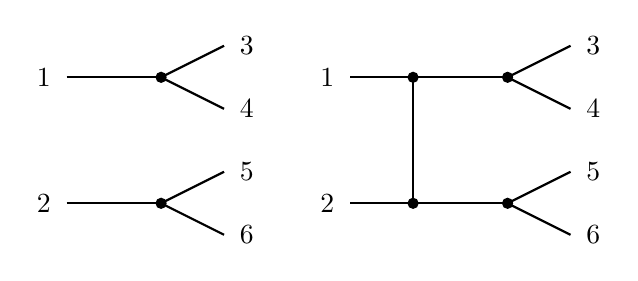
\begin{tikzpicture}[scale=0.8, thick]

                % ==========================================
                % LEFT SIDE: Disconnected Diagrams
                % ==========================================

                % Coordinates for the left diagrams
                \coordinate (L1)  at (0, 2);
                \coordinate (L2)  at (0, 0);
                \coordinate (Lv1) at (1.5, 2); % Upper interaction vertex
                \coordinate (Lv2) at (1.5, 0); % Lower interaction vertex
                \coordinate (L3)  at (2.5, 2.5);
                \coordinate (L4)  at (2.5, 1.5);
                \coordinate (L5)  at (2.5, 0.5);
                \coordinate (L6)  at (2.5, -0.5);

                % Upper disconnected piece (1 -> 3,4)
                \draw (L1) -- (Lv1);
                \draw (Lv1) -- (L3);
                \draw (Lv1) -- (L4);

                % Lower disconnected piece (2 -> 5,6)
                \draw (L2) -- (Lv2);
                \draw (Lv2) -- (L5);
                \draw (Lv2) -- (L6);

                % External states labels
                \node[left=2pt]  at (L1) {\(1\)};
                \node[left=2pt]  at (L2) {\(2\)};
                \node[right=2pt] at (L3) {\(3\)};
                \node[right=2pt] at (L4) {\(4\)};
                \node[right=2pt] at (L5) {\(5\)};
                \node[right=2pt] at (L6) {\(6\)};

                % Interaction vertices dots
                \filldraw (Lv1) circle (2pt);
                \filldraw (Lv2) circle (2pt);


                % ==========================================
                % RIGHT SIDE: Connected Diagram
                % ==========================================

                % Coordinates for the right diagram (shifted leftwards for better spacing)
                \coordinate (R1)   at (4.5, 2);
                \coordinate (R2)   at (4.5, 0);
                \coordinate (Rv1a) at (5.5, 2); % First upper vertex
                \coordinate (Rv2a) at (5.5, 0); % First lower vertex
                \coordinate (Rv1b) at (7, 2);   % Splitting upper vertex
                \coordinate (Rv2b) at (7, 0);   % Splitting lower vertex
                \coordinate (R3)   at (8, 2.5);
                \coordinate (R4)   at (8, 1.5);
                \coordinate (R5)   at (8, 0.5);
                \coordinate (R6)   at (8, -0.5);

                % Upper connected line
                \draw (R1) -- (Rv1a) -- (Rv1b);
                \draw (Rv1b) -- (R3);
                \draw (Rv1b) -- (R4);

                % Lower connected line
                \draw (R2) -- (Rv2a) -- (Rv2b);
                \draw (Rv2b) -- (R5);
                \draw (Rv2b) -- (R6);

                % Internal vertical propagator connecting the two parts
                \draw (Rv1a) -- (Rv2a);

                % External states labels
                \node[left=2pt]  at (R1) {\(1\)};
                \node[left=2pt]  at (R2) {\(2\)};
                \node[right=2pt] at (R3) {\(3\)};
                \node[right=2pt] at (R4) {\(4\)};
                \node[right=2pt] at (R5) {\(5\)};
                \node[right=2pt] at (R6) {\(6\)};

                % Interaction vertices dots
                \filldraw (Rv1a) circle (2pt);
                \filldraw (Rv2a) circle (2pt);
                \filldraw (Rv1b) circle (2pt);
                \filldraw (Rv2b) circle (2pt);

            \end{tikzpicture}
        \end{minipage}
        \hfill
        \begin{minipage}{0.35\textwidth}
            \caption{In the calculation of scattering amplitudes and fully interacting correlation functions, disconnected sub-diagrams (left) are factored out and excluded. Only fully connected topologies (right) contribute to the non-trivial S-matrix elements.}
        \end{minipage}
        \label{fig:connected_vs_disconnected}
    \end{figure}
    The non fully connected diagram describes to separate processes more than a global interaction of 2 incoming particles scattering into 4 outgoing particles, and thus it does not contribute to the scattering amplitude of the process we are interested in, while the fully connected diagram describes exactely the process we are interested in.
\end{example}

\begin{remark}
    At leading order we have set \(Z=1\), and we confused the lagrangian mass with the physical one: in the next chapter we will see that at higher order corrections we need to take into account the renormalization of the theory, which will lead us to distinguish between the lagrangian mass and the physical mass, and to introduce a renormalization factor \(Z\) for the fields:
    \[
        \begin{dcases}
            Z = 1 + \mathcal{O}(\lambda), \\
            m_\text{phys} = m_{\mathcal{L}} + \mathcal{O}(\lambda).
        \end{dcases}
    \]
    this will modify the Feynman rules we have just described, but for now we can ignore these complications and use the rules we have just derived. In our Feynman rules we are using the lagrangian mass \(m_{\mathcal{L}}\), but in future it will be convenient to make the substitution \(m_{\mathcal{L}} \to m_\text{phys} + \delta m\), where \(\delta m\) represents additional terms added to the lagrangian.
\end{remark}

\subsubsection{Back to LSZ Reduction Formula}

Now consider a \(2 \to n\) scattering process, where we have two incoming particles and \(n\) outgoing particles.
\begin{figure}[H]
    \centering
    \tikzset{
        directed/.style={
                postaction={decorate},
                decoration={
                        markings,
                        mark=at position 0.6 with {\arrow{stealth}}
                    }
            },
        blackbox/.style={
                circle,
                draw=black,
                minimum size=1cm,
                fill=white,
                pattern=north east lines,
                pattern color=black!60,
                thick
            }
    }
    \begin{tikzpicture}[scale=1, thick]

        \node[blackbox] (blob) at (0,0) {};

        \coordinate (in_coords) at (-2.5, 0);

        \draw[directed, orange!90!black] (in_coords |- 0, 1) -- (blob.160);
        \node[orange!90!black, left, font=\mathstrut] at (in_coords |- 0, 1) {$p_a$};

        \draw[directed, orange!90!black] (in_coords |- 0, -1) -- (blob.200);
        \node[orange!90!black, left, font=\mathstrut] at (in_coords |- 0, -1) {$p_b$};


        \coordinate (out_coords) at (2.5, 0);

        \draw[directed, green!80!black] (blob.40) -- (out_coords |- 0, 1);
        \node[green!80!black, right, font=\mathstrut] at (out_coords |- 0, 1) {$p_1$};

        \draw[directed, green!80!black] (blob.20) -- (out_coords |- 0, 0.3);
        \node[green!80!black, right, font=\mathstrut] at (out_coords |- 0, 0.3) {$p_2$};

        \draw[directed, green!80!black] (blob.340) -- (out_coords |- 0, -0.3);
        \node[green!80!black, text height=1ex, text depth=0.1ex] at (2.8, -0.5) {$\vdots$};

        \draw[directed, green!80!black] (blob.320) -- (out_coords |- 0, -1);
        \node[green!80!black, right, font=\mathstrut] at (out_coords |- 0, -1) {$p_n$};

    \end{tikzpicture}
\end{figure}
If we want to calculate the scattering amplitude for this process, we can use the LSZ reduction formula, which relates the S-matrix element to the Green's function. The Green's function we need to calculate is given by
\[
    \dots
\]

We have seen thay at leading order (LO) we have \(Z=1\) and in the LSZ reduction formula we have a factor of \(\prod_{j=1}^{n+2} \left( -i(p_j^2 - m^2) \right)\), where \(p_j\) are the external momenta, which are on-shell, thus they satisfy the mass-shell condition \(p_j^2 = m^2\) for \(j=1,2,\ldots,n+2\). This means that each of the external lines contributing with a factor of \(-i(p_j^2 - m^2)\) cancels with a factor of \(\frac{i}{p_j^2 - m^2}\) from the propagator of the internal line.

But what happens at higher order corrections? We can schematically represent the contribution of the diagrams to the scattering amplitude as follows:

\begin{figure}[H]
    \begin{minipage}{0.6\textwidth}
        \centering
        \begin{tikzpicture}[scale=0.7, thick]

            % ==========================================
            % 1. DEFINE STYLES
            % ==========================================
            % Style for the central "Amputated" blob
            \tikzstyle{amputatedBlob} = [draw, thick, ellipse, minimum width=3cm, minimum height=1.5cm, align=center, font=\mathstrut\bfseries]

            % Style for the full propagator corrections (hatched bubbles)
            \tikzstyle{propBubble1} = [circle, draw, thick, minimum size=0.6cm, pattern=north east lines, pattern color=orange!90!black]
            \tikzstyle{propBubble2} = [circle, draw, thick, minimum size=0.6cm, pattern=north east lines, pattern color=green!80!black]


            % ==========================================
            % 2. CENTRAL BLOB
            % ==========================================
            \node[amputatedBlob] (blob) at (0,0) {AMPUTATED};

            % ==========================================
            % 3. LEFT SIDE (Incoming momenta p_A, p_B)
            % ==========================================
            % Hatched bubbles
            \node[propBubble1] (bA) at (-4, 1) {};
            \node[propBubble1] (bB) at (-4, -1) {};

            % External momentum labels
            \node[left=4pt, font=\mathstrut, orange!90!black] (pA) at (-5.5, 1.3) {\(p_a\)};
            \node[left=4pt, font=\mathstrut, orange!90!black] (pB) at (-5.5, -1.3) {\(p_b\)};

            % Draw connecting lines
            \draw[orange!90!black] (pA) -- (bA);
            \draw[orange!90!black] (bA) -- (blob.155); % .155 connects to the top-left edge of the ellipse

            \draw[orange!90!black] (pB) -- (bB);
            \draw[orange!90!black] (bB) -- (blob.205); % .205 connects to the bottom-left edge

            % ==========================================
            % 4. RIGHT SIDE (Outgoing momenta p_1, p_2, ..., p_N)
            % ==========================================
            % Hatched bubbles
            \node[propBubble2] (b1) at (4, 1.2) {};
            \node[propBubble2] (b2) at (4, 0) {};
            \node[propBubble2] (bN) at (4, -1.4) {};

            % External momentum labels
            \node[right=4pt, font=\mathstrut, green!80!black] (p1) at (5.5, 1.4) {\(p_1\)};
            \node[right=4pt, font=\mathstrut, green!80!black] (p2) at (5.5, 0) {\(p_2\)};
            \node[right=4pt, font=\mathstrut, green!80!black] (pN) at (5.5, -1.6) {\(p_n\)};

            % Draw connecting lines
            \draw[green!80!black] (blob.25) -- (b1);  % Top right connection
            \draw[green!80!black] (b1) -- (p1);

            \draw[green!80!black] (blob.0) -- (b2);   % Middle right connection
            \draw[green!80!black] (b2) -- (p2);

            \draw[green!80!black] (blob.335) -- (bN); % Bottom right connection
            \draw[green!80!black] (bN) -- (pN);

            % ==========================================
            % 5. VERTICAL DOTS (For the N lines)
            % ==========================================
            % Placed between the second and N-th outgoing lines
            \node[font=\small, green!80!black] at (5.8, -0.6) {\(\vdots\)}; % Dots near the labels
            \node[font=\small, green!80!black] at (4, -0.6) {\(\vdots\)};   % Dots between the bubbles

        \end{tikzpicture}
    \end{minipage}
    \hfill
    \begin{minipage}{0.35\textwidth}
        \caption{Structure of a fully interacting correlation function. To obtain the S-matrix element, the external legs containing the full propagator corrections (hatched circles) are amputated, leaving only the amputated connected Green's function in the center.}
    \end{minipage}
    \label{fig:amputated_diagram}
\end{figure}
\begin{equation*}
    \text{Where:} \quad
    \begin{cases}
        \quad \legFullProp \quad = \quad \text{sum of 2-point diagrams,} \\[20pt]
        \quad \legAmputated \quad = \quad \text{sum of ``amputated diagrams''}
    \end{cases}
\end{equation*}

\begin{definition}[Amputated diagram]
    \uline{An amputated diagram is a Feynman diagram where we cannot disconnect any external line by cutting a single internal line}. In other words, an amputated diagram is a diagram that does not contain any disconnected subdiagram, and thus it is fully connected.

    The contribution of an amputated diagram to the scattering amplitude is given by the \textit{product of the propagators corresponding to the internal lines}, and the \textit{factors from the vertexes}, without including the external propagators, since they are on-shell and thus they do not contribute to the scattering amplitude.
\end{definition}

\begin{example}
    In the following diagram, we have a cut procedure used to amputate a 1-loop self-energy correction from an incoming external leg. Thanks to the LSZ reduction formalism, we know that the external legs of the Green's function contain full propagator corrections, which are given by the sum of all the 2-point diagrams, and thus we can amputate them in order to extract more efficiently the scattering amplitude: we will see how we are ignoring self-deleting terms, since in the computation of the green's function in the LSZ reduction formula these contributions cancel out.
    \begin{figure}[H]
        \begin{minipage}{0.5\textwidth}
            \centering
            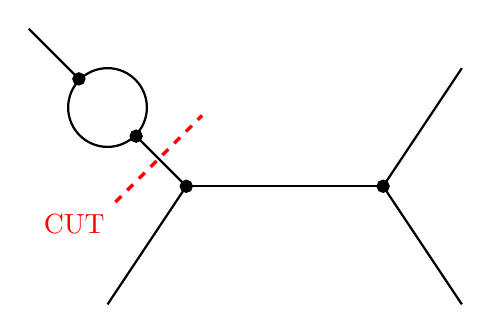
\begin{tikzpicture}[scale=1, thick]
                % 1. Drawing the 1-Loop Bubble
                \tikzstyle{Bubble} = [circle, draw, thick, minimum size=1cm]
                \node[Bubble] (loop) at (-1, 1) {};

                % 2. Coordinate Definitions
                % Central main vertices
                \coordinate (VL) at (0,0);
                \coordinate (VR) at (2.5,0);

                % Right-side outgoing external legs
                \coordinate (OutTop) at (3.5, 1.5);
                \coordinate (OutBot) at (3.5, -1.5);

                % Left-side bottom incoming leg
                \coordinate (InBot) at (-1, -1.5);

                % Left-side top incoming leg (with the loop)
                \coordinate (LoopBot) at (loop.315);
                \coordinate (LoopTop) at (loop.135);
                \coordinate (InTop)   at (-2, 2);

                % 3. Drawing Propagators
                \draw (VL) -- (VR);          % Internal s-channel propagator
                \draw (VR) -- (OutTop);      % Top right leg
                \draw (VR) -- (OutBot);      % Bottom right leg
                \draw (VL) -- (InBot);       % Bottom left leg
                \draw (VL) -- (LoopBot);     % Line connecting main vertex to the loop
                \draw (LoopTop) -- (InTop);  % Far external top-left leg

                % 4. Drawing Interaction Nodes (Dots)
                \filldraw (VL) circle (2pt);
                \filldraw (VR) circle (2pt);
                \filldraw (LoopBot) circle (2pt);
                \filldraw (LoopTop) circle (2pt);

                % 5. The "CUT" dashed line
                \draw[red, dashed, very thick] (-0.9, -0.2) -- (0.2, 0.9)
                node[pos=0, below left, font=\mathstrut] {CUT};

            \end{tikzpicture}
        \end{minipage}
        \hfill
        \begin{minipage}{0.45\textwidth}
            \caption{Example of a cutting procedure used to amputate a 1-loop self-energy correction from an incoming external leg. In the LSZ reduction formalism, isolating and removing these external full-propagator corrections is required to extract the pure amputated scattering amplitude.}
            \label{fig:amputation_cut}
        \end{minipage}%
    \end{figure}
\end{example}

Let us show that the contribution of the external subdiagrams we are amputating is negligible for the scattering amplitude. Each of the external lines in the LSZ reduction contributes with a factor
\[
    -\frac{i}{\sqrt{Z}}\left( p_j^2 - m^2 \right),
\]
and we know these momenta to be on-shell, thus they satisfy the mass-shell condition \(p_j^2 = m^2\) for \(j=1,2,\ldots,n+2\) (\(m\) is the physical mass). Thus each of the external subdiagrams we are truncating is the sum of two point functions:
\[
    \begin{aligned}
        p_j \, \to \, \feynBlobNE & = \feynBare + \feynBlobEmpty + \feynBlobVert + \dots                                        \\
                                  & = \text{ Fourier transform of } \bra{\Omega} T \hat{\phi}(x_1) \hat{\phi}(x_2) \ket{\Omega} \\
                                  & = \frac{i Z}{p_j^2 - m^2} + \text{ regular terms at } p_j^2 \sim m^2,
    \end{aligned}
\]
which implies that each of the \(\tfrac{i}{p_j^2 - m^2}\) terms cancel with the \(-i(p_j^2 - m^2)\) factor from the LSZ reduction formula, leaving us with a factor of \(\sqrt{Z}\) for each external line, which is the pole residue of the full propagator.

\subsubsection{Summary of Rules in Momentum Space}

\begin{itemize}
    \item \(i \mathcal{M} = \sum\) fully connected amputated diagrams.
    \item Assign momentum to internal lines, with the convention that the momentum flows from the initial state to the final state, and it is conserved at each vertex.
    \item For each unresolved momentum, i.e. for each loop, we need to integrate over it with the measure \(\int \frac{\mathrm{d}^4 k}{(2\pi)^4}\).
    \item External lines contribute with a factor of 1 each, since they are on-shell and thus they do not contribute to the scattering amplitude.
    \item Internal lines contribute with a factor of \(\frac{i}{p^2 - m^2}\) each, where \(p\) is the momentum flowing through the internal line: propagator \(\equiv\) internal line.
    \item Vertexes contribute with a factor of \(-i \lambda\) for a \(\phi^3\) theory, and more generally by the Fourier transform of the interaction term in the Lagrangian, which depends on the theory under consideration and on the momenta flowing through the vertex.
    \item The symmetry factor of the diagram is given by \(1/S\), where \(S\) is the number of symmetries of the diagram, which can be calculated by counting the number of ways to permute the vertexes and fields without changing the diagram.
    \item For each external particle, we need to multiply by a factor of \(\sqrt{Z}\), which comes from the LSZ reduction formula: \(Z\) is the pole residue of the full propagator, and it is equal to 1 at the leading order, but it can receive corrections at higher orders.
\end{itemize}

We derived these feynman rules from a real scalar theory with a cubic interaction, but they can be easily generalized to other theories: the only theory specific point is the vertex factor, which depends on the interaction term in the Lagrangian, while the other rules are general and can be applied to any theory.